\documentclass[shortpres,usenames,dvipsnames]{beamer}
\usetheme{CambridgeUS}

% Depending on build configuration, one of these packages will
% enable unicode
\usepackage[utf8]{inputenc}
\usepackage{fontspec}
\usepackage{listings}

%Images
\usepackage{graphics}
\usepackage{graphicx, svg}
\usepackage{caption}
\usepackage{adjustbox}

%Mixed
\usepackage{subfig}
\usepackage{multicol}
\usepackage{xcolor}
\usepackage{colortbl}
\usepackage{pgfplots}
\usepackage{xmpmulti}
\usepackage{verbatim}
\usepackage{array}
\usepackage{tabularx}
\usepackage{cprotect}

%Tikz
\usepackage{tikz}
\usepackage{environ}
\usetikzlibrary{positioning}



\usepackage{algorithm,algpseudocode}  %for algorithm environmenstacle in the bathymetry to show the effect of the soruce terms in 2D.t

\setbeamertemplate{footline}
{
	\leavevmode%
	\hbox{%
		\begin{beamercolorbox}[wd=.333333\paperwidth,ht=2.25ex,dp=1ex,center]{author in head/foot}%
			\usebeamerfont{author in head/foot}\insertshortauthor%~~\beamer@ifempty{\insertshortinstitute}{}{(\insertshortinstitute)}
		\end{beamercolorbox}%
		\begin{beamercolorbox}[wd=.333333\paperwidth,ht=2.25ex,dp=1ex,center]{title in head/foot}%
			\usebeamerfont{title in head/foot}\insertshorttitle
		\end{beamercolorbox}%
		\begin{beamercolorbox}[wd=.333333\paperwidth,ht=2.25ex,dp=1ex,right]{date in head/foot}%
			\usebeamerfont{date in head/foot}\insertshortdate{}\hspace*{2em}
			\insertframenumber{} / \inserttotalframenumber\hspace*{2ex}
		\end{beamercolorbox}}%
		\vskip0pt%
	}\part{title}
	\beamertemplatenavigationsymbolsempty
	
	
	%color specification---------------------------------------------------------------
	\definecolor{TUMblue}{rgb}{0.00, 0.40, 0.74}
	\definecolor{TUMgray}{rgb}{0.85, 0.85, 0.86}
	\definecolor{TUMpantone285C}{rgb}{0.00, 0.45, 0.81}
	\definecolor{lightblue}{rgb}{0.7529,0.8118,0.9333}
	
	\setbeamercolor{block title}{fg=white, bg=TUMpantone285C}
	\setbeamercolor{block body}{bg=lightblue}
	\setbeamertemplate{blocks}[rounded][shadow=true]
	%----------------------------------------------------------------------------------
	
	\setbeamercolor{frametitle}{fg=TUMblue, bg=white}
	\setbeamercolor{palette primary}{fg=TUMblue,bg=TUMgray}
	\setbeamercolor{palette secondary}{use=palette primary,fg=TUMblue,bg=white}
	\setbeamercolor{palette tertiary}{use=palette primary,fg=white, bg=TUMblue}
	\setbeamercolor{palette quaternary}{use=palette primary,fg=white,bg=TUMpantone285C}
	
	
	\setbeamercolor{title}{bg=white,fg=TUMblue}
	\setbeamercolor{item projected}{use=item,fg=black,bg = lightblue}
	\setbeamercolor{block title}{fg=black, bg=lightblue}
	\setbeamercolor{block body}{bg=white}
	\setbeamertemplate{blocks}[rounded][shadow=true]
	%----------------------------------------------------------------------------------
	
	
	%############### Self defined commands ##############################
	\newcommand{\imgvoffset}{-20pt}
	\newcommand{\texthoffset}{20pt}
	\newcommand{\imgfullscale}{0.75}
	\newcommand{\imgcolscale}{0.9}
	
	\captionsetup[subfigure]{labelformat=empty}		%Disable enumeration of subfigures
	%####################################################################
	
	%############### Title information ###############
	\title[{Tsunami simulation}]{Project}
	\author[Bellamy, Honal, Wieser]{Gruppe 03\\George Bellamy, Christoph Honal, Felix Wieser\\\vspace{10pt}{\small Bachelorpraktikum}}
	\institute[TU M\"unchen]{Technical University of Munich}
	\date{9. Januar 2018}
	%#################################################
	
	%############### Tikz picture configuration ###############
	\newcommand{\pgfglobalscale}{0.7}
	\newcommand{\pgfglobalheadervspace}{\vspace{5pt}\\}
	%##########################################################
	
	\lstset{escapeinside={<@}{@>}}
	
	\begin{document}
		\maketitle
		
%TODO change pictures		
		
\begin{frame}{Overview}
	\begin{figure}
		\subfloat[User Interface \tiny **]{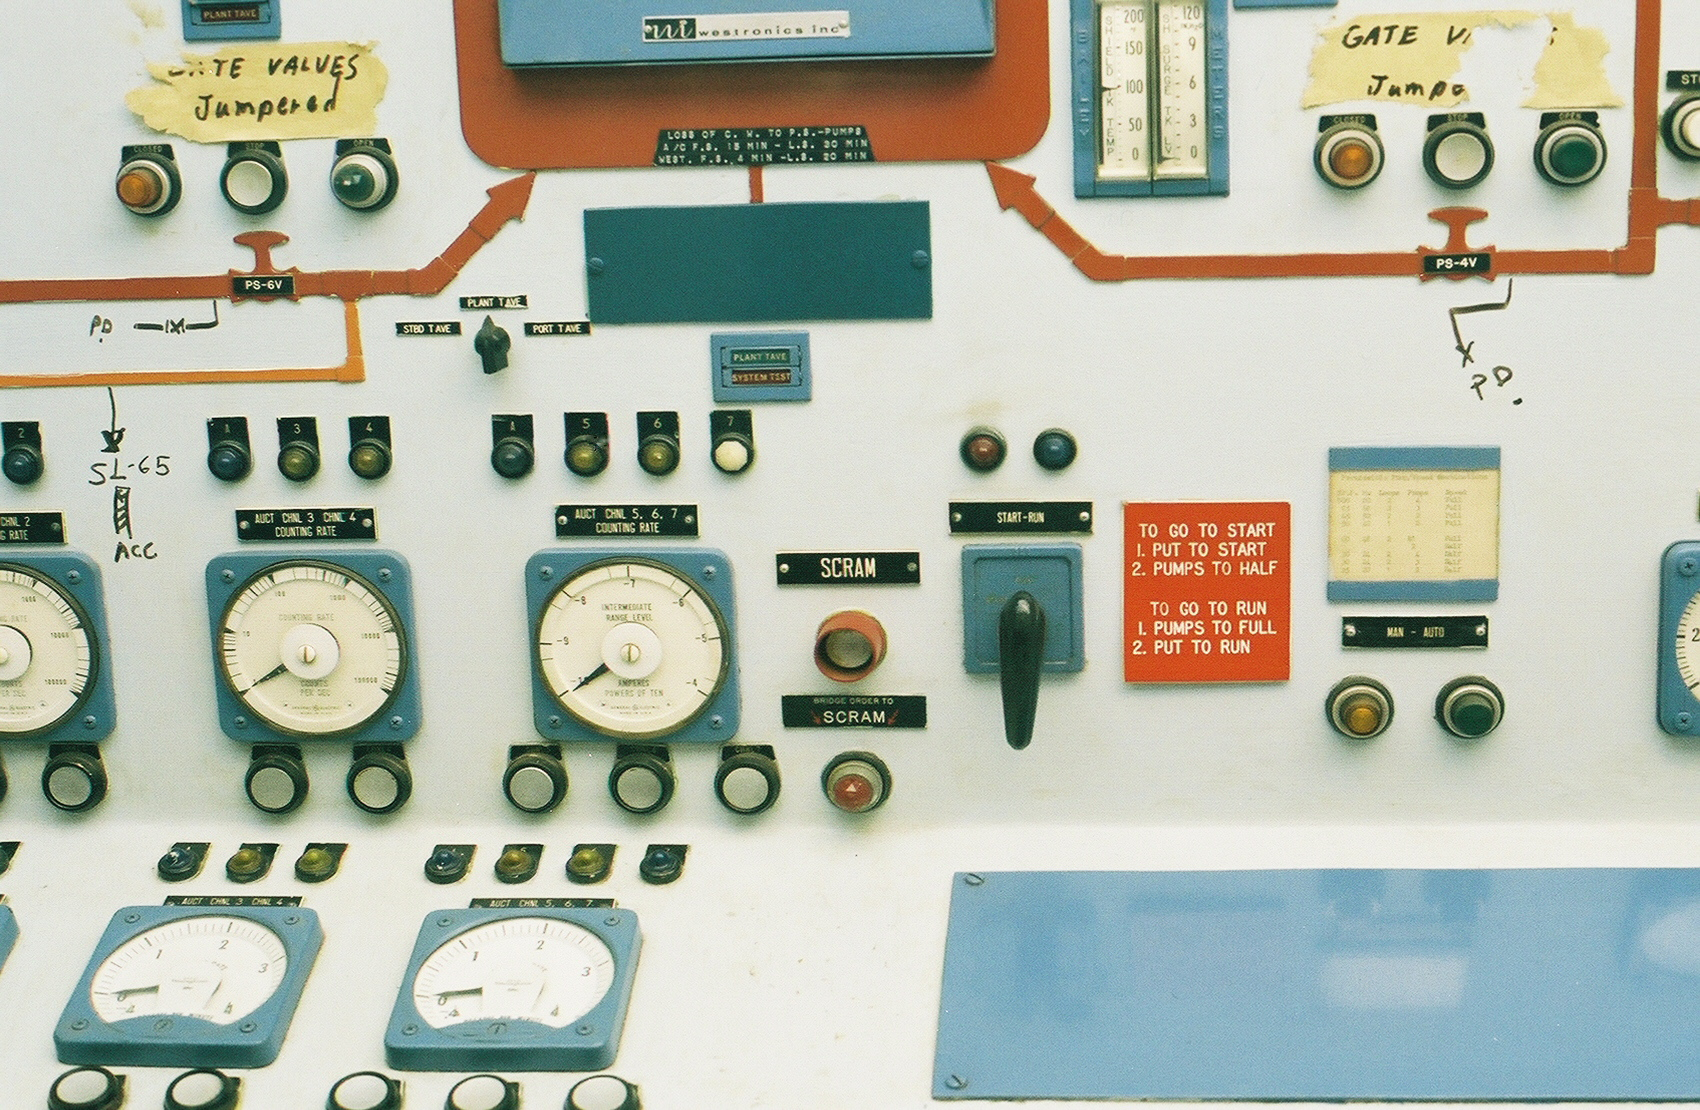
\includegraphics[clip,width=0.3\linewidth]
			{img/UI_old.jpg}}
		\hspace{20pt}
		\subfloat[Backend \tiny *]{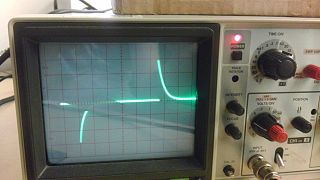
\includegraphics[clip,width=0.3\linewidth]
			{img/oszi.jpg}}
		\hspace{40pt}\vspace{10pt}\\
		\subfloat[Demonstration]{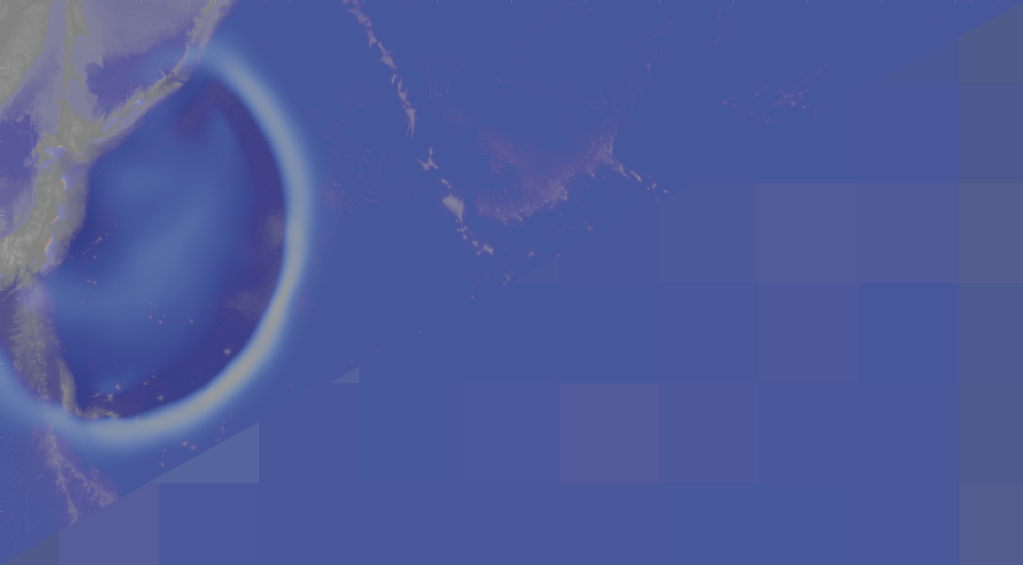
\includegraphics[clip,width=0.3\linewidth]
			{img/tuhoku_mixed.png}}
		\vfill
		\flushleft
		{\fontsize{5}{5} \selectfont *Image: \url{https://commons.wikimedia.org/wiki/File:1tt.jpg}}
		\flushleft
		{\fontsize{5}{5} \selectfont **Image: \url{https://upload.wikimedia.org/wikipedia/commons/e/e8/NS_Savannah_-_Reactor_Control_Panel_-_SCRAM_Button.jpg}}
	\end{figure}
\end{frame}

\begin{frame}[fragile]{UI}
	\begin{figure}
		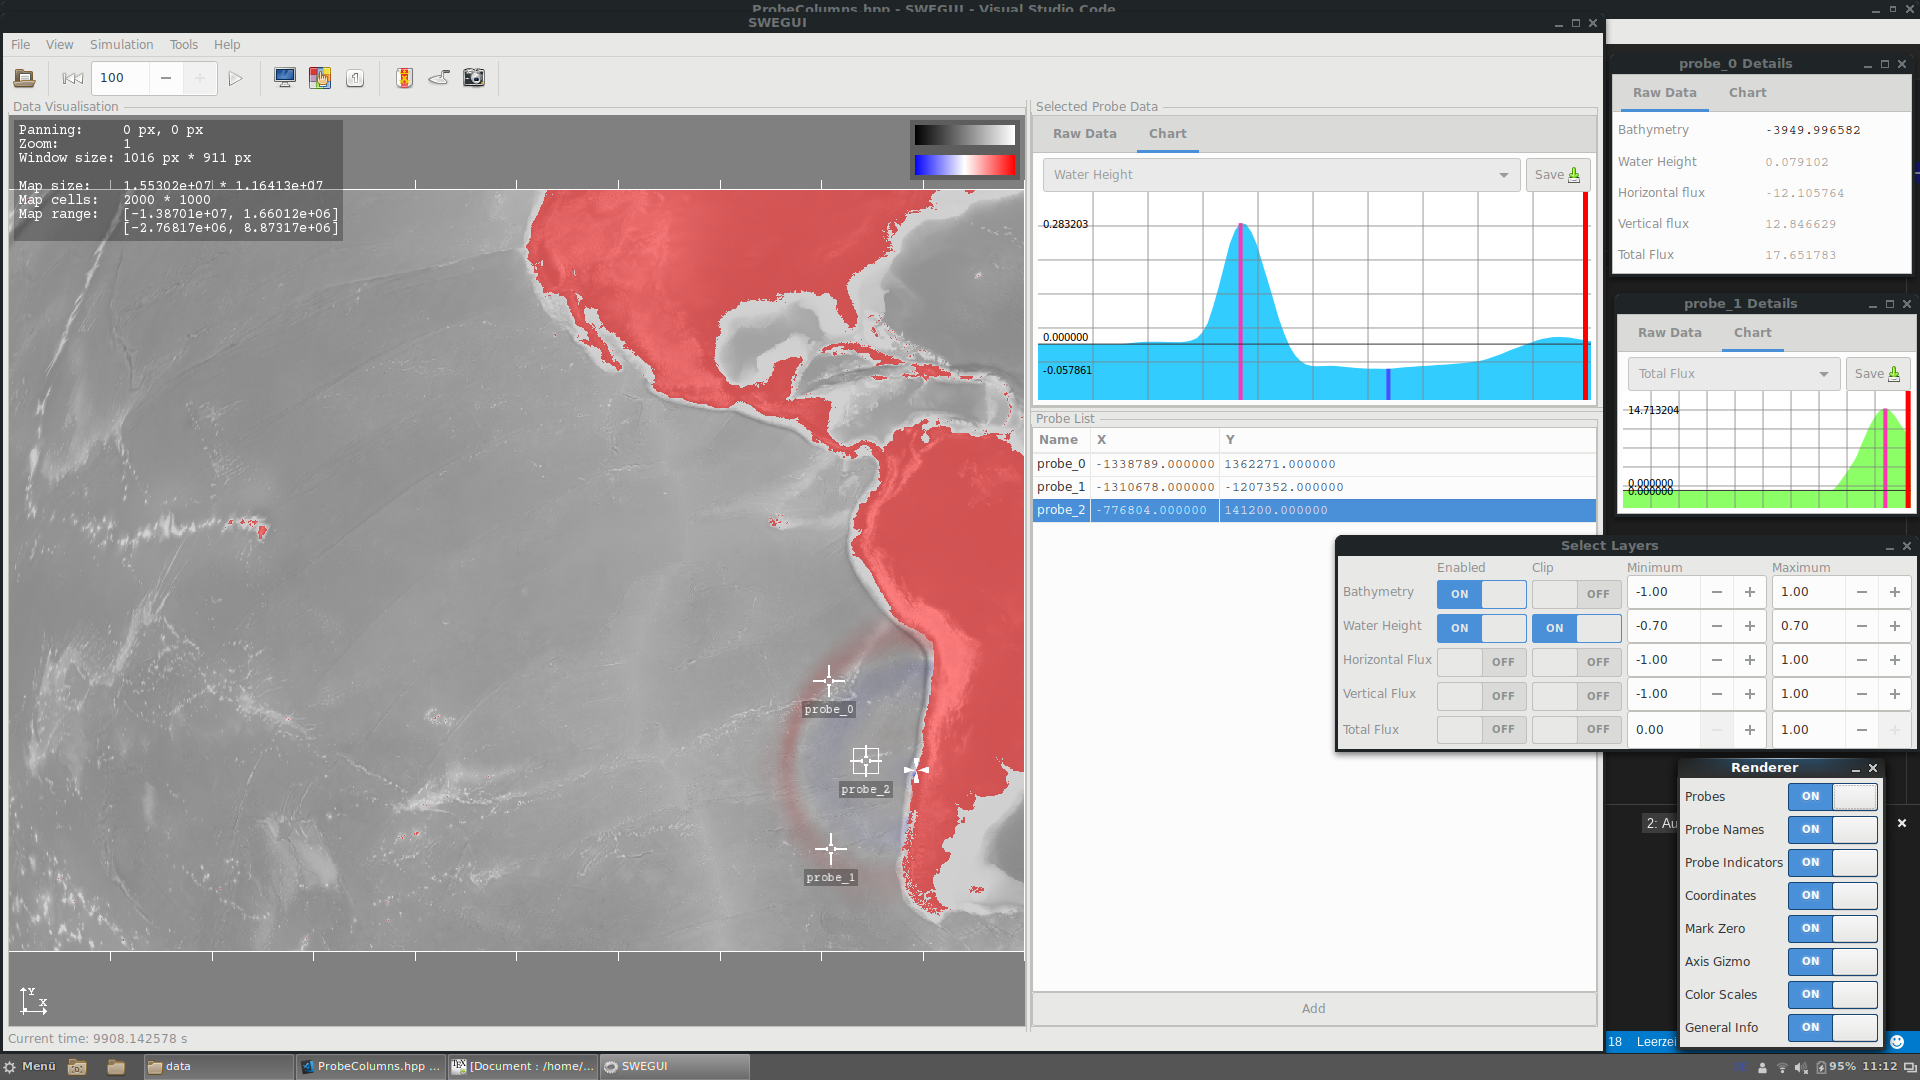
\includegraphics[clip, width=\linewidth]{img/screenshot_1.png}
	\end{figure}
\end{frame}

\begin{frame}[fragile]{Toolbar}
	\begin{figure}
		
\includegraphics[clip, width=60mm]{img/toolbar.png}
	\end{figure}
	\begin{itemize}
		\item Open new files (NetCDF)
		\item Control the simulation step
		\item Open layer selection
	\end{itemize}
\end{frame}

\begin{frame}[fragile]{Data visualisation}
	\begin{figure}
		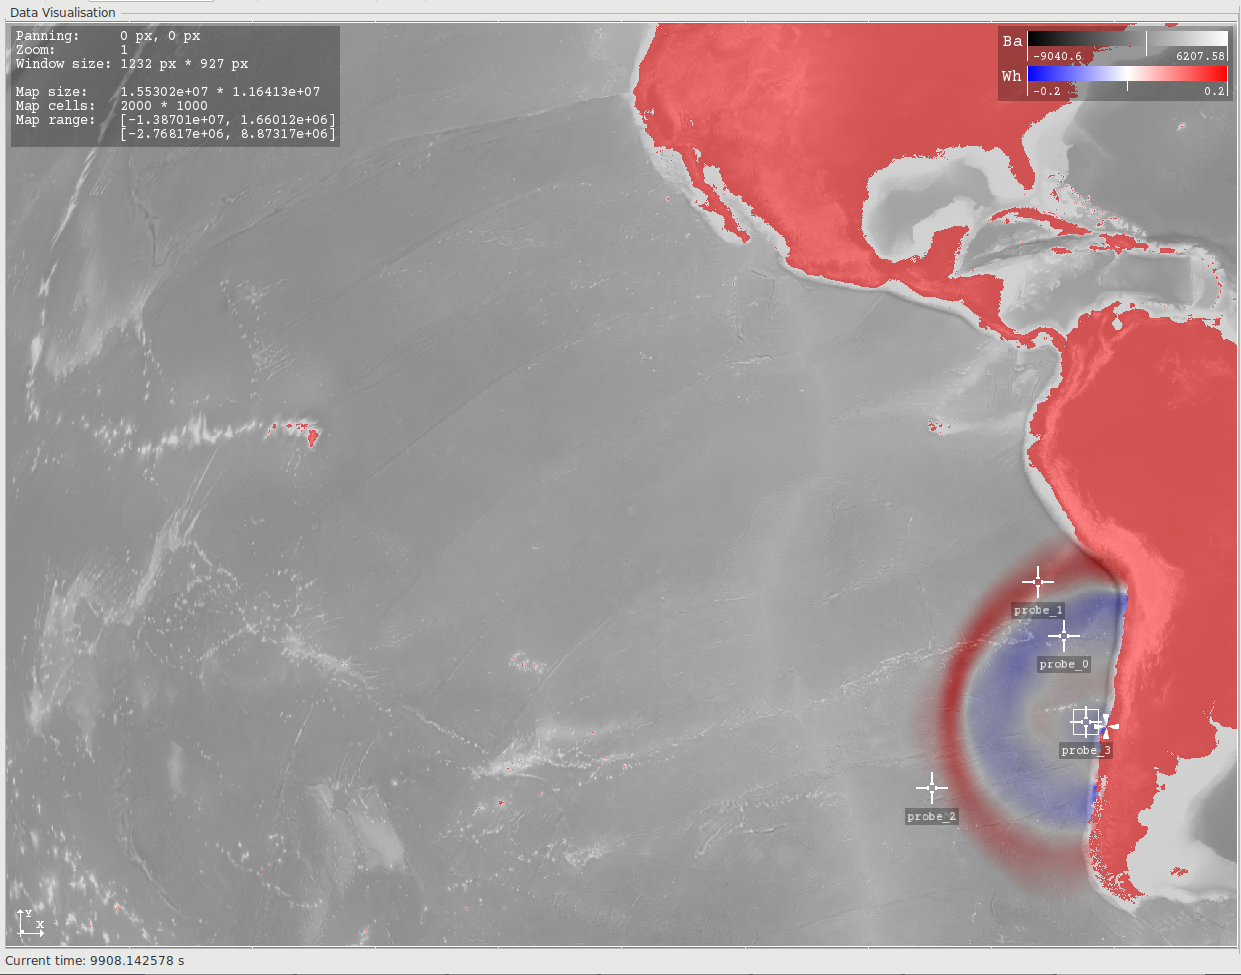
\includegraphics[clip, width=80mm]{img/datavis.png}
	\end{figure}
	\begin{itemize}
		\item Color shading is chosen according to the max/min values
		\item Probes are shown as crosshaires
		\item Different data sets can be displayed
	\end{itemize}
\end{frame}

\begin{frame}[fragile]{Layer selection}
	\begin{figure}
		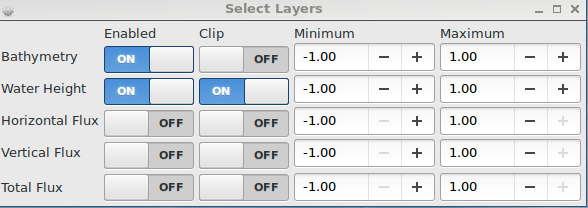
\includegraphics[clip, width=80mm]{img/layerselect.png}
	\end{figure}
	\begin{itemize}
		\item Choose between data sets
		\item Clip displayed range to visualize small changes
	\end{itemize}
\end{frame}

\begin{frame}[fragile]{Probes}
	\begin{figure}
		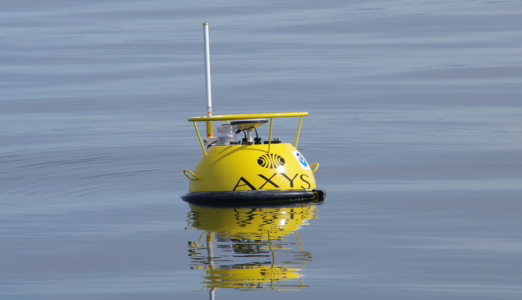
\includegraphics[clip, width=80mm]{img/Buoy.jpg}
	\end{figure}
	\begin{itemize}
		\item Select a point in the data visualization or create one with its coordinates
		\item Points can be selected and their information is shown
		\item Custom naming for probes
	\end{itemize}
	\vfill
	\flushleft
	{\fontsize{5}{5} \selectfont \url{http://axystechnologies.com/wp-content/uploads/2013/09/HydroLevel-Mini-Buoy-IT.jpg}}
\end{frame}

\begin{frame}[fragile]{Data display}
	\begin{figure}
		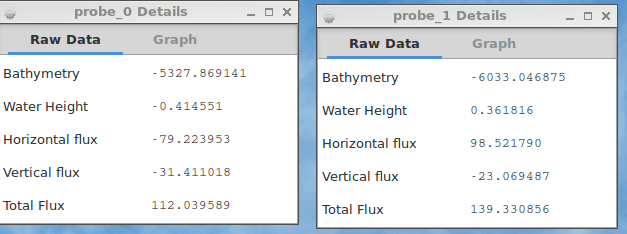
\includegraphics[clip, width=80mm]{img/datadisplay.png}
	\end{figure}
	\begin{itemize}
		\item Display probe data
		\item Optional extra windows to monitor multiple probes
	\end{itemize}
\end{frame}


\begin{frame}[fragile]{Graphs}
	\begin{figure}
		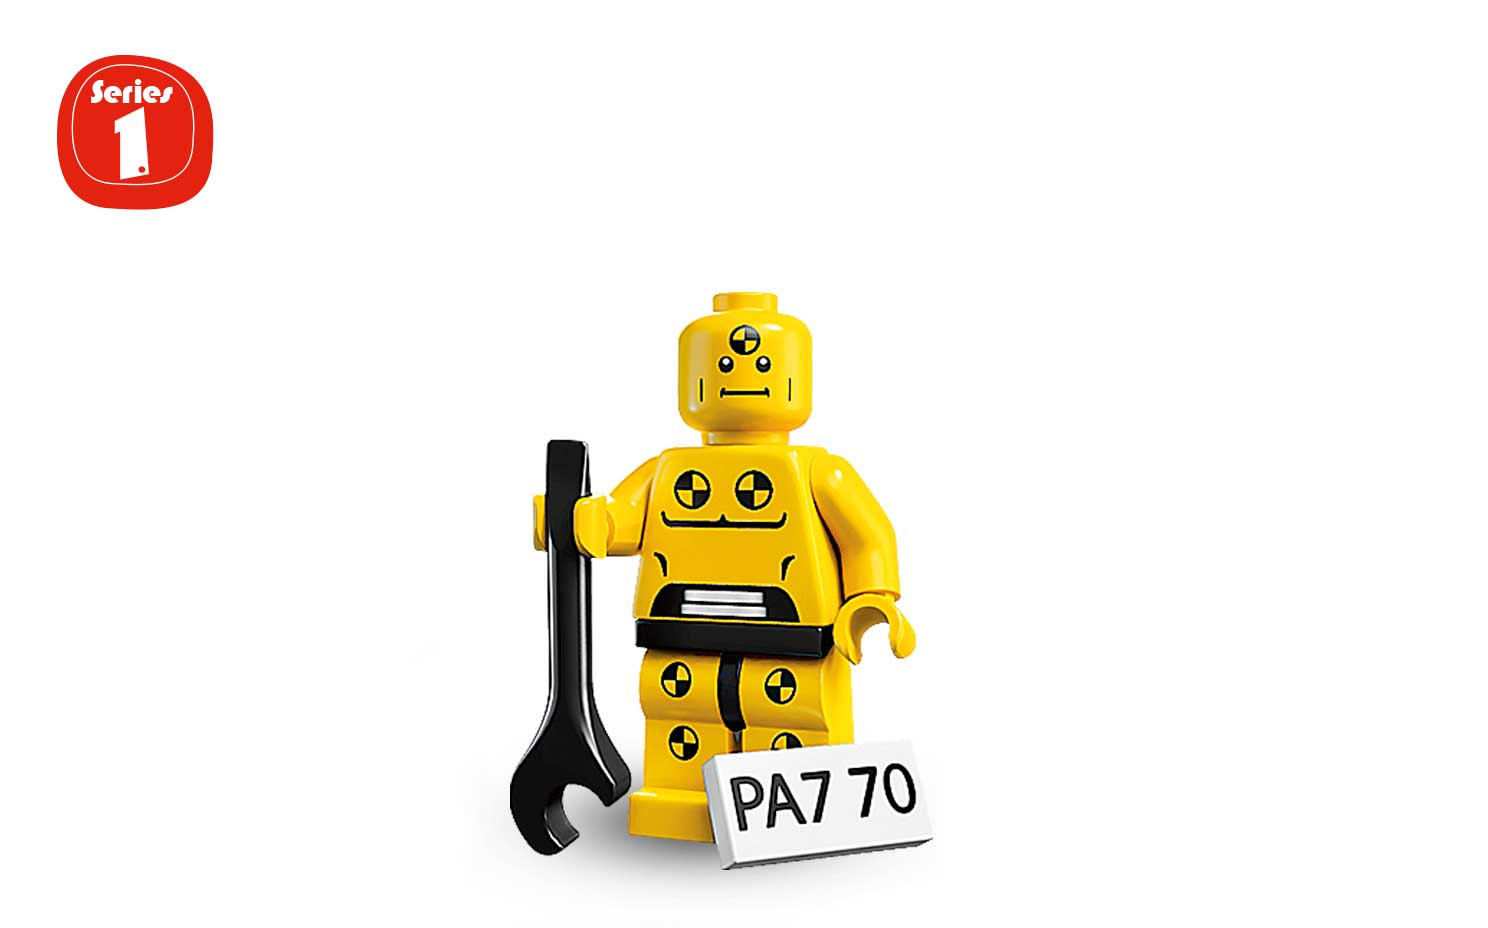
\includegraphics[clip, width=80mm]{img/dummy_image.jpg}
	\end{figure}
	\begin{itemize}
		\item Click two points on the rendered view and the cross section between these two is selected
		\item A separate window shows the cross section graph
		\item Screen shots of these can be exported
	\end{itemize}
\end{frame}

\begin{frame}[fragile]{UI implementation - toolset}
	\begin{figure}
		
\includegraphics[clip, width=20mm]{img/GTK_logo.png}
	\end{figure}
	\textbf{gtkmm for C++}
	\begin{itemize}
		\item Easy to use library 
		\item Based on gtk UI, used in gimp originally
		\item Rendered view is done by shader, all UI is gtkmm
		\item Toolbar icons and interface are integrated in to gtkmm 
	\end{itemize}
	\vfill
	\flushleft
	{\fontsize{5}{5} \selectfont \url{https://de.wikipedia.org/wiki/Gtkmm#/media/File:GTK2B_logo.svg}}
\end{frame}
	
\begin{frame}[fragile]{UI implementation - toolset}
	\begin{figure}
		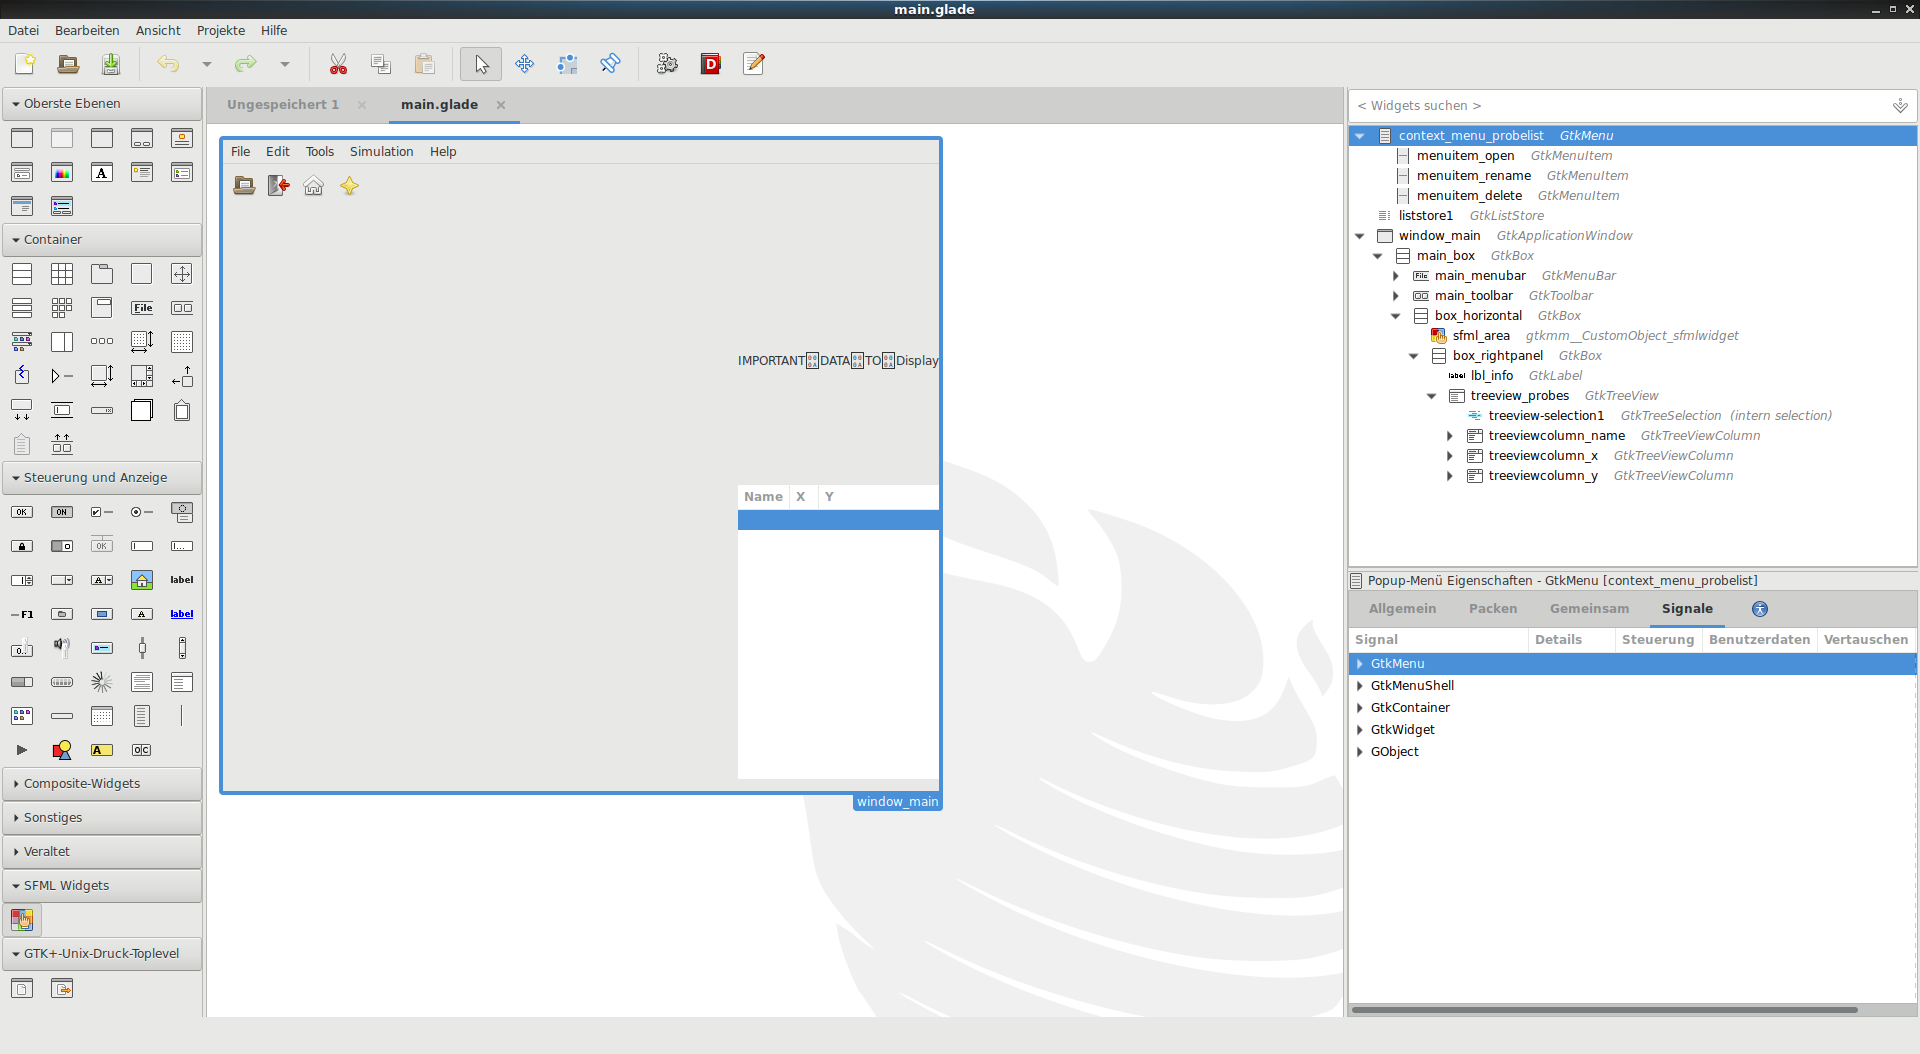
\includegraphics[clip, width=75mm]{img/glade.png}
	\end{figure}
	\textbf{glade}\\
	\begin{itemize}
		\item WYSIWYG interface editor 
		\item Generates an XML which describes the UI
		\item The UI is built with an extra widget for the renderer
	\end{itemize}
\end{frame}

\begin{frame}[fragile]{Shader implementation - toolset}
	\begin{figure}
		
\includegraphics[clip, width=50mm]{img/sfml.png}
	\end{figure}
	\textbf{SFML}\\
	\begin{itemize}
		\item openGL interface
		\item Rendering view uses openGL to display data
	\end{itemize}
	\vfill
	\flushleft
	{\fontsize{5}{5} \selectfont \url{https://upload.wikimedia.org/wikipedia/commons/thumb/b/bf/SFML2.svg/230px-SFML2.svg.png}}
\end{frame}

\begin{frame}[fragile]{Shader implementation - transport encoding}
	\begin{figure}
		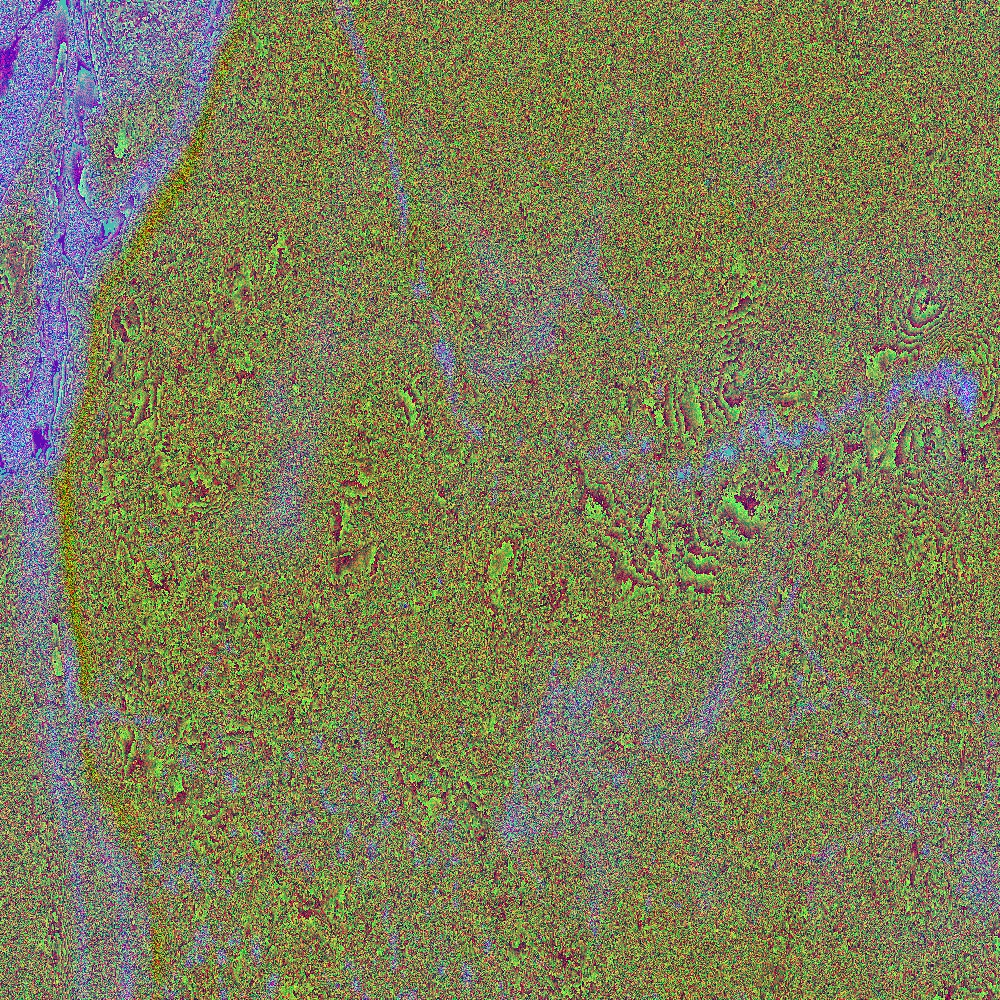
\includegraphics[clip, width=50mm]{img/transport_encoding.jpg}
	\end{figure}
	\begin{itemize}
		\item Encode float to RGB double for renderer
	\end{itemize}
\end{frame}


\begin{frame}[fragile]{Code Structure}
bla
\end{frame}

\begin{frame}[fragile]{Demonstration}
	\begin{figure}
		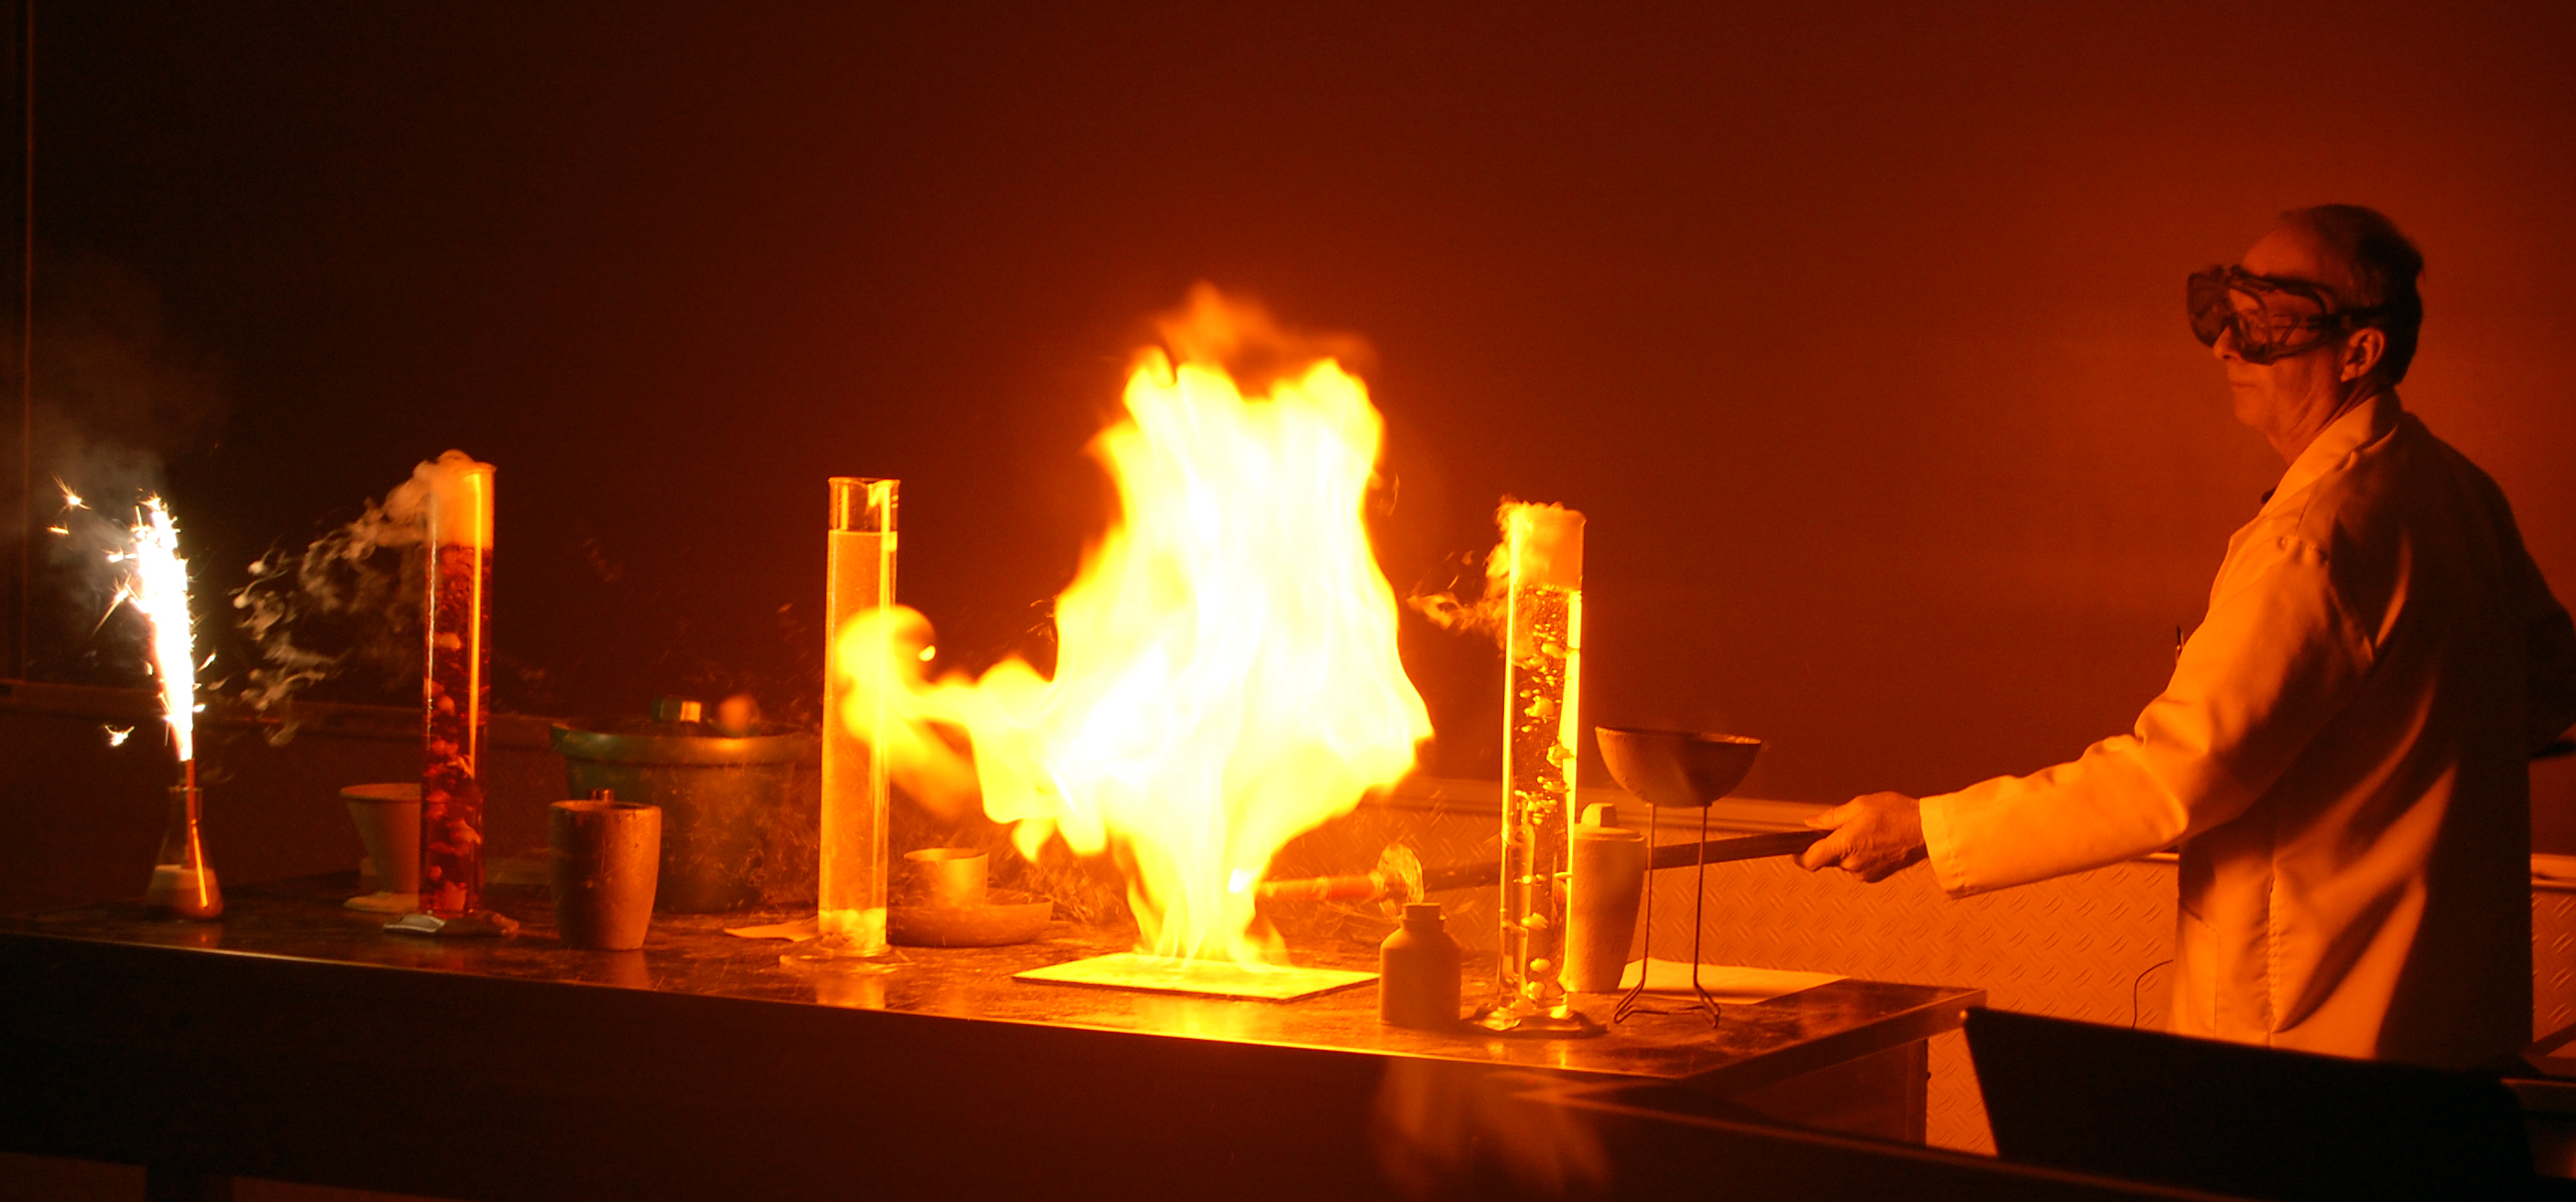
\includegraphics[clip, width=\linewidth]{img/demo.jpeg}
	\end{figure}
	
	\vfill
	\flushleft
	{\fontsize{5}{5} \selectfont \url{https://news.uns.purdue.edu/images/2012/chemistry-show.jpg}}
\end{frame}

\begin{frame}{}
	\begin{figure}
		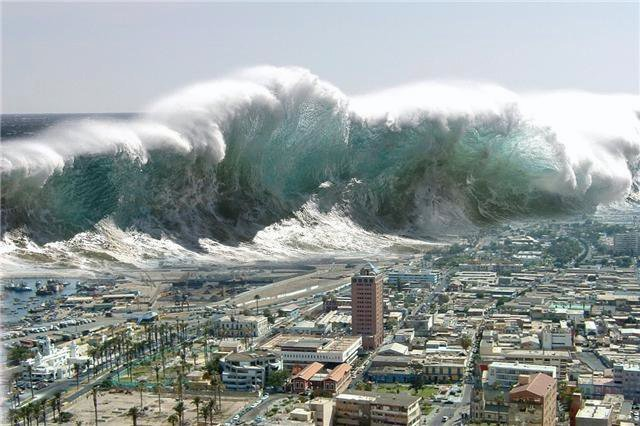
\includegraphics[clip, width=\imgfullscale\linewidth]{img/tsunami.jpg}
	\end{figure}
	\centering
	\vspace{10pt}
	Thank you for your attention
	\\
	\vfill
	\flushleft
	{\fontsize{5}{5} \selectfont \url{http://userscontent2.emaze.com/images/88c09d66-4283-49c0-9f80-9eb8fd05e30f/16101782-ea98-4b06-b114-4637be705926.jpg}}
\end{frame}
\end{document}